\clearpage



\appendix

\section{Regression figures}\label{app:regression}

\begin{figure}[h!]
    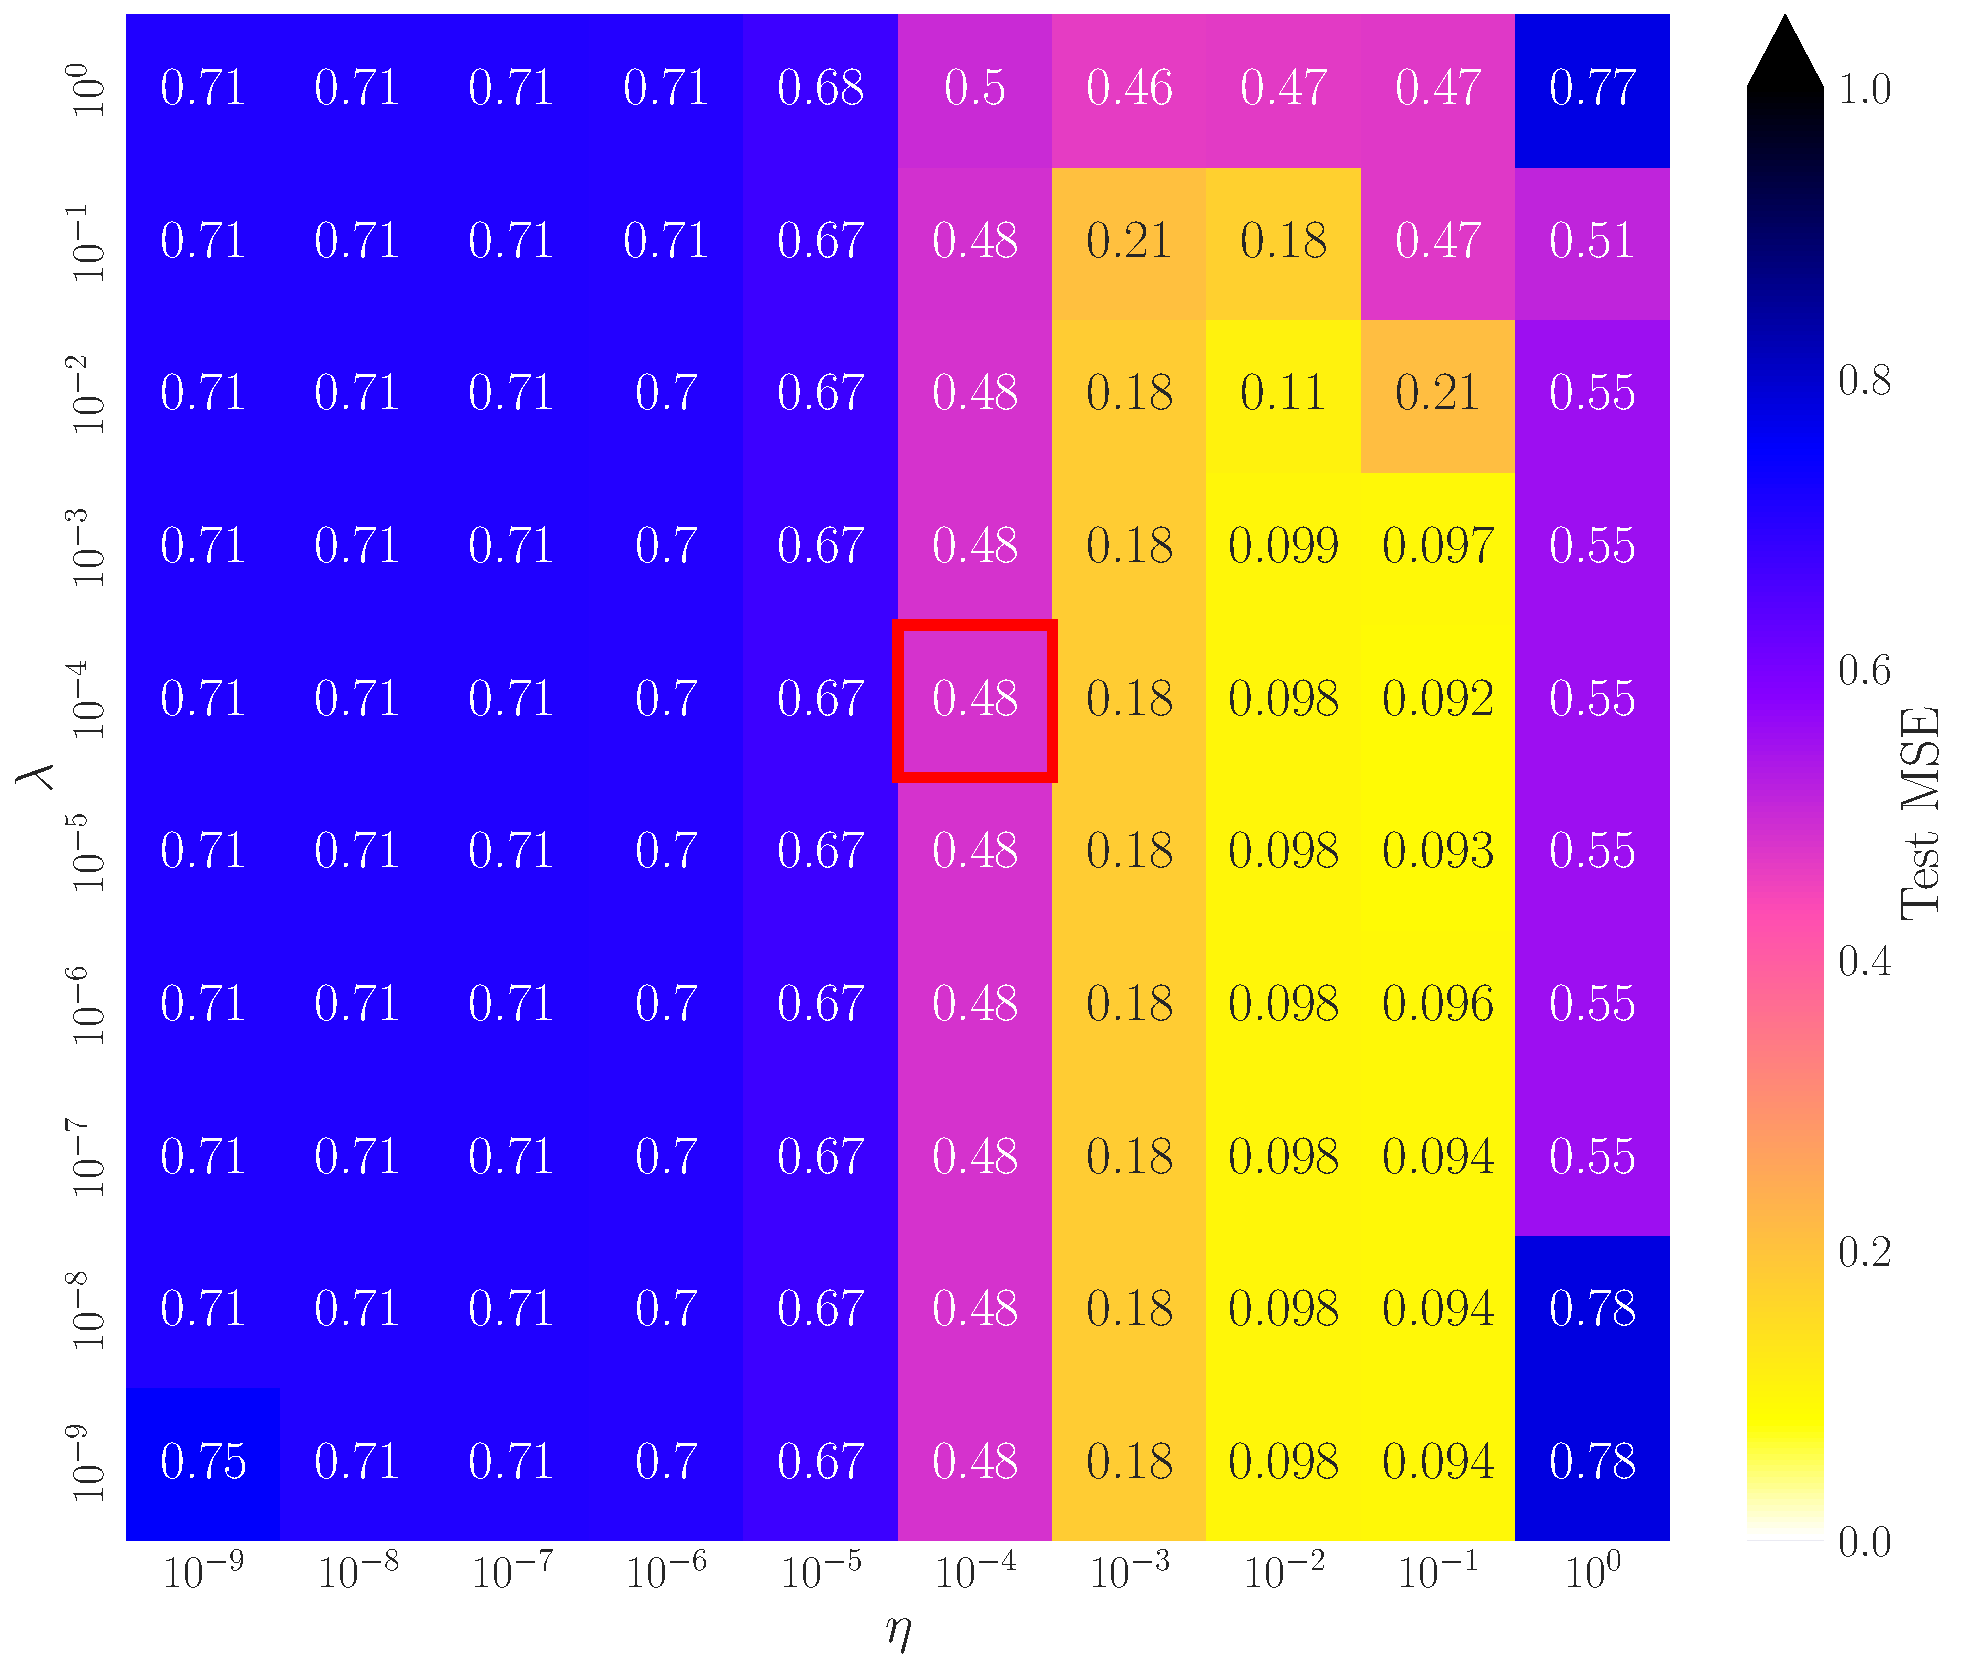
\includegraphics[width=\linewidth]{eta_lambda_analysis.pdf}
    \caption{Heatmap of the MSE as function of learning rate $\eta$ and regularisation parameter $\lambda$, using SGD with RMSProp as optimiser performing regression analysis of a 3 layered, 15-10-5 neurons, neural network. }
    \label{fig:reg_eta_lambda}
\end{figure}

\begin{figure}[h!]
    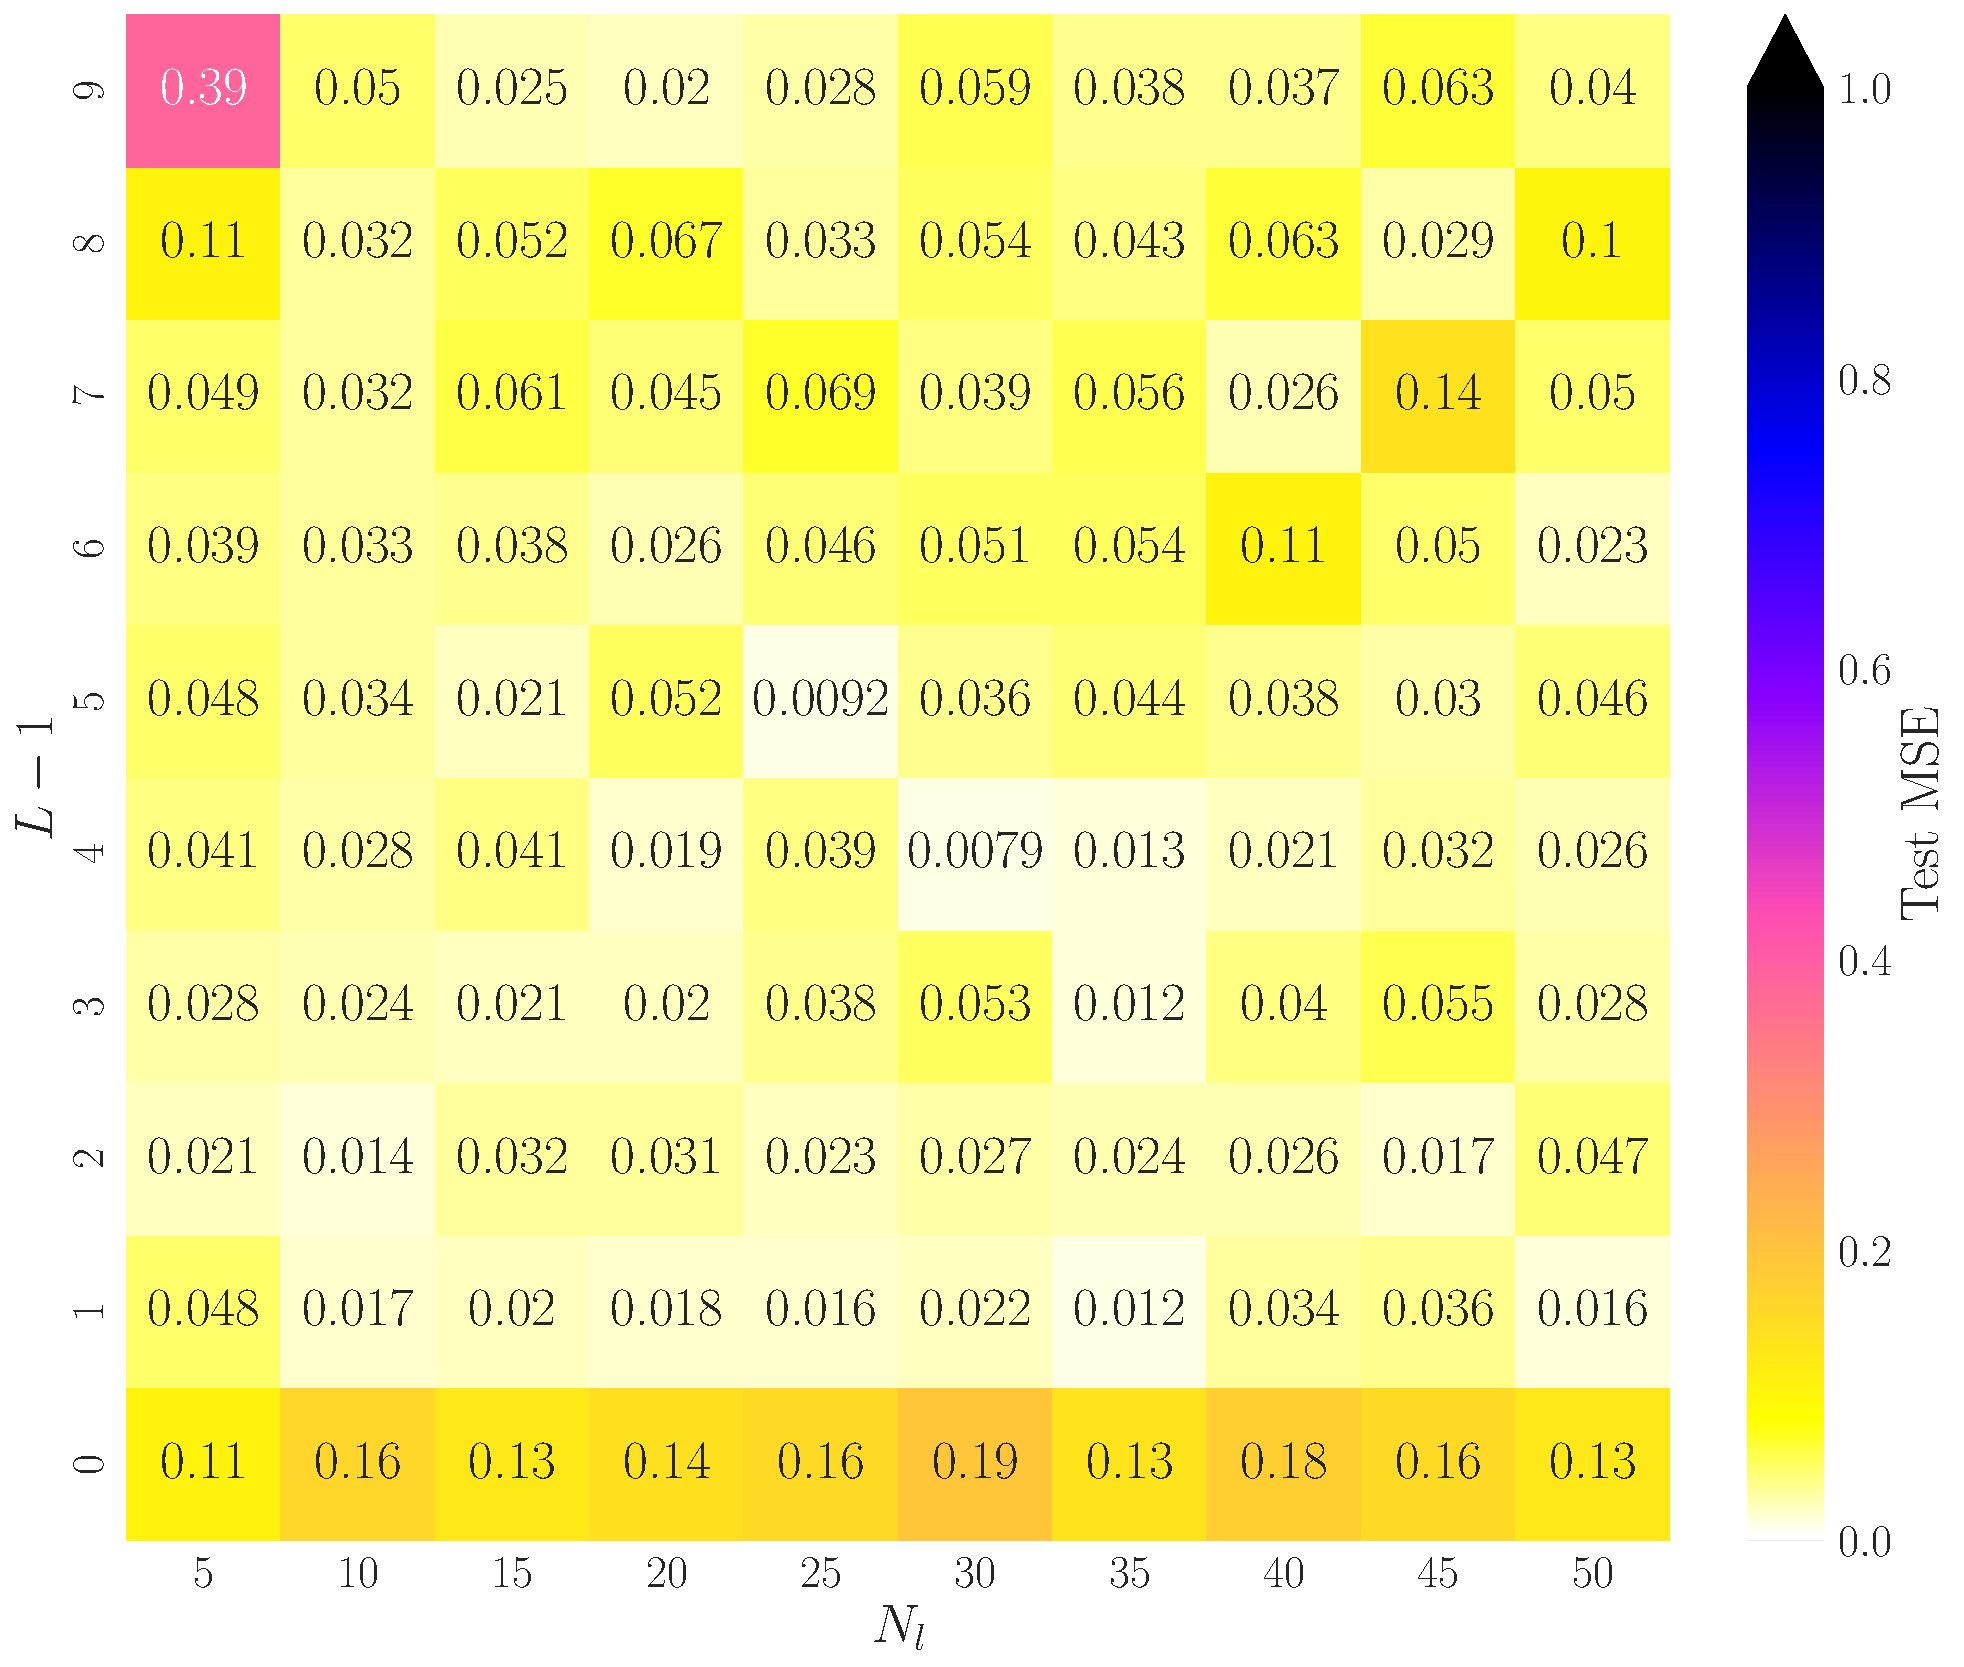
\includegraphics[width=\linewidth]{layer_neuron_analysis.pdf}
    \caption{Heatmap of the MSE as function of hidden layers $L-1$ and neurons per layer $N_l$, using SGD with RMSProp as optimiser performing regression analysis with $\eta=10^{-1}$ and $\lambda=10^{-4}$.}
    \label{fig:reg_layer_neuron}
\end{figure}

\begin{figure}[h!]
    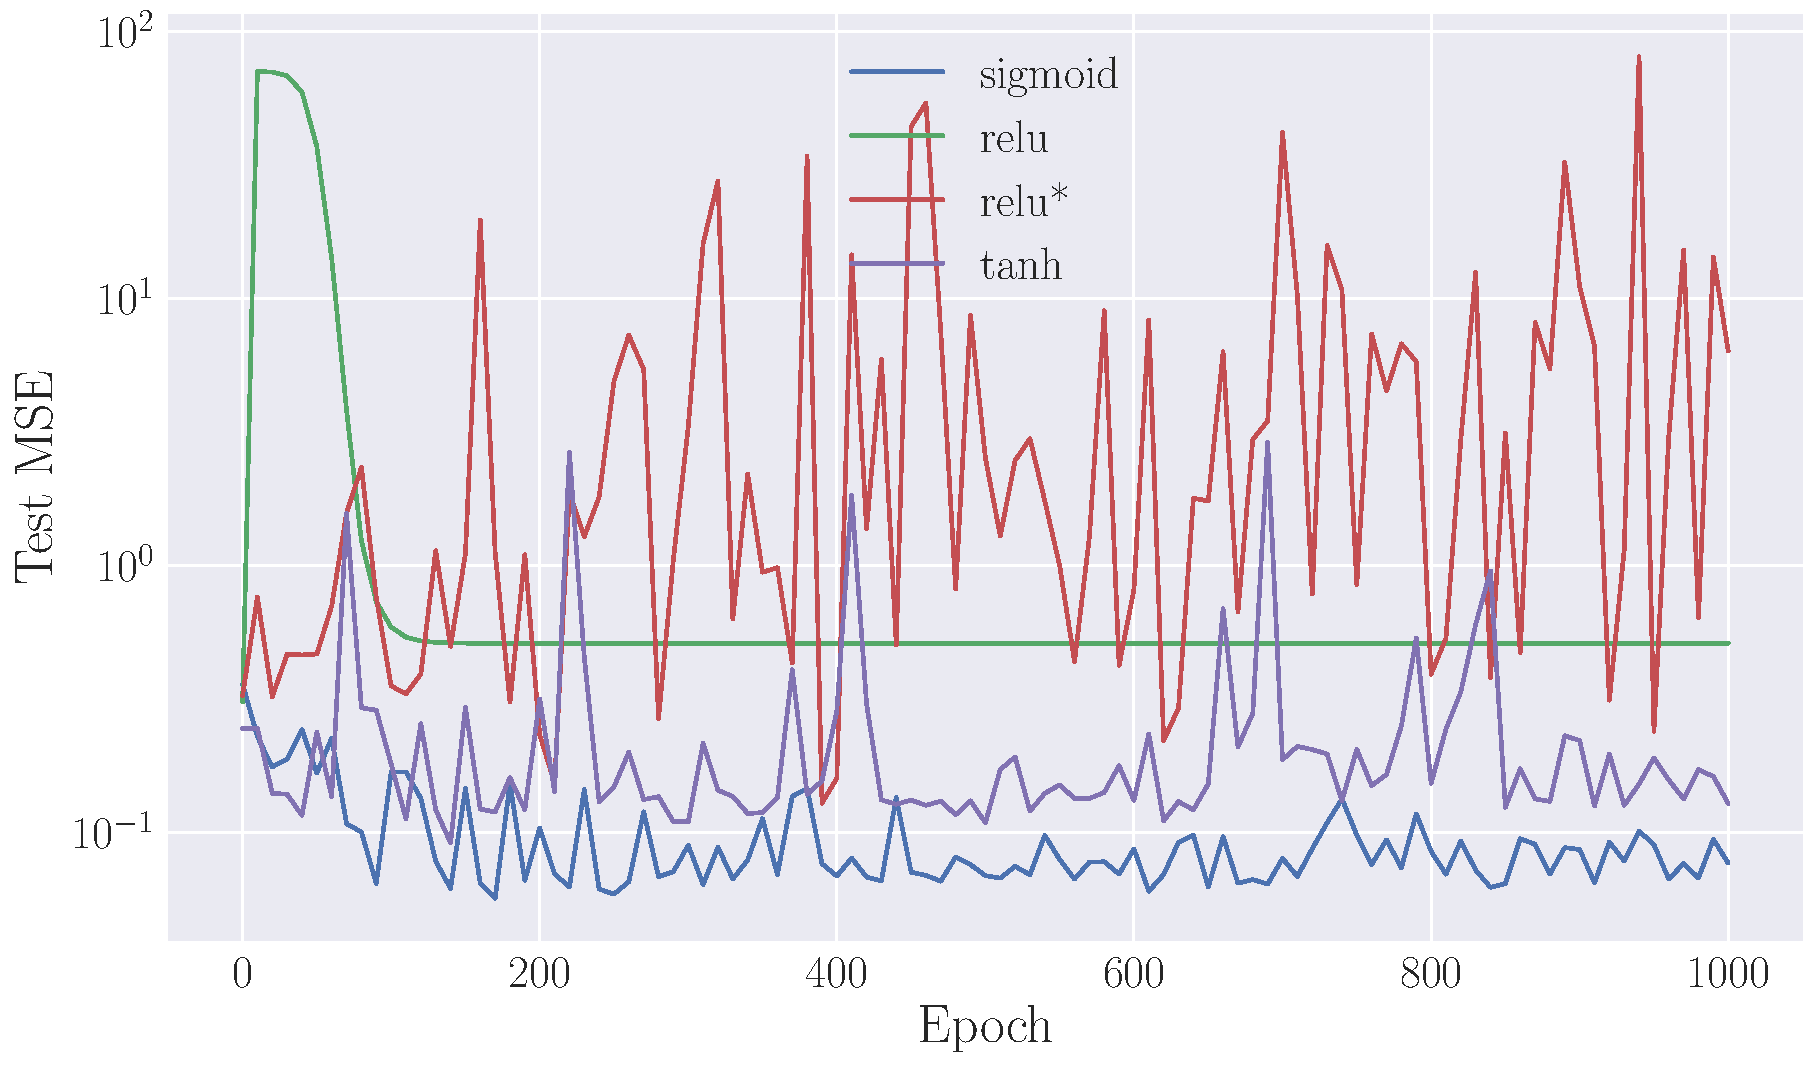
\includegraphics[width=\linewidth]{actFuncPer1000Epoch.pdf}
    \caption{Plot of the MSE for up to 1000 epochs, using SGD with RMSProp as optimiser performing regression analysis with $L-1=1$ hidden layer with $N_l=30$ neurons with $\eta=10^{-1}$ and $\lambda=10^{-4}$. The four different activation functions perform differently. Note the logarithmic MSE axis.}
    \label{fig:reg_act_epoch1000}
\end{figure}

\begin{figure}[h!]
    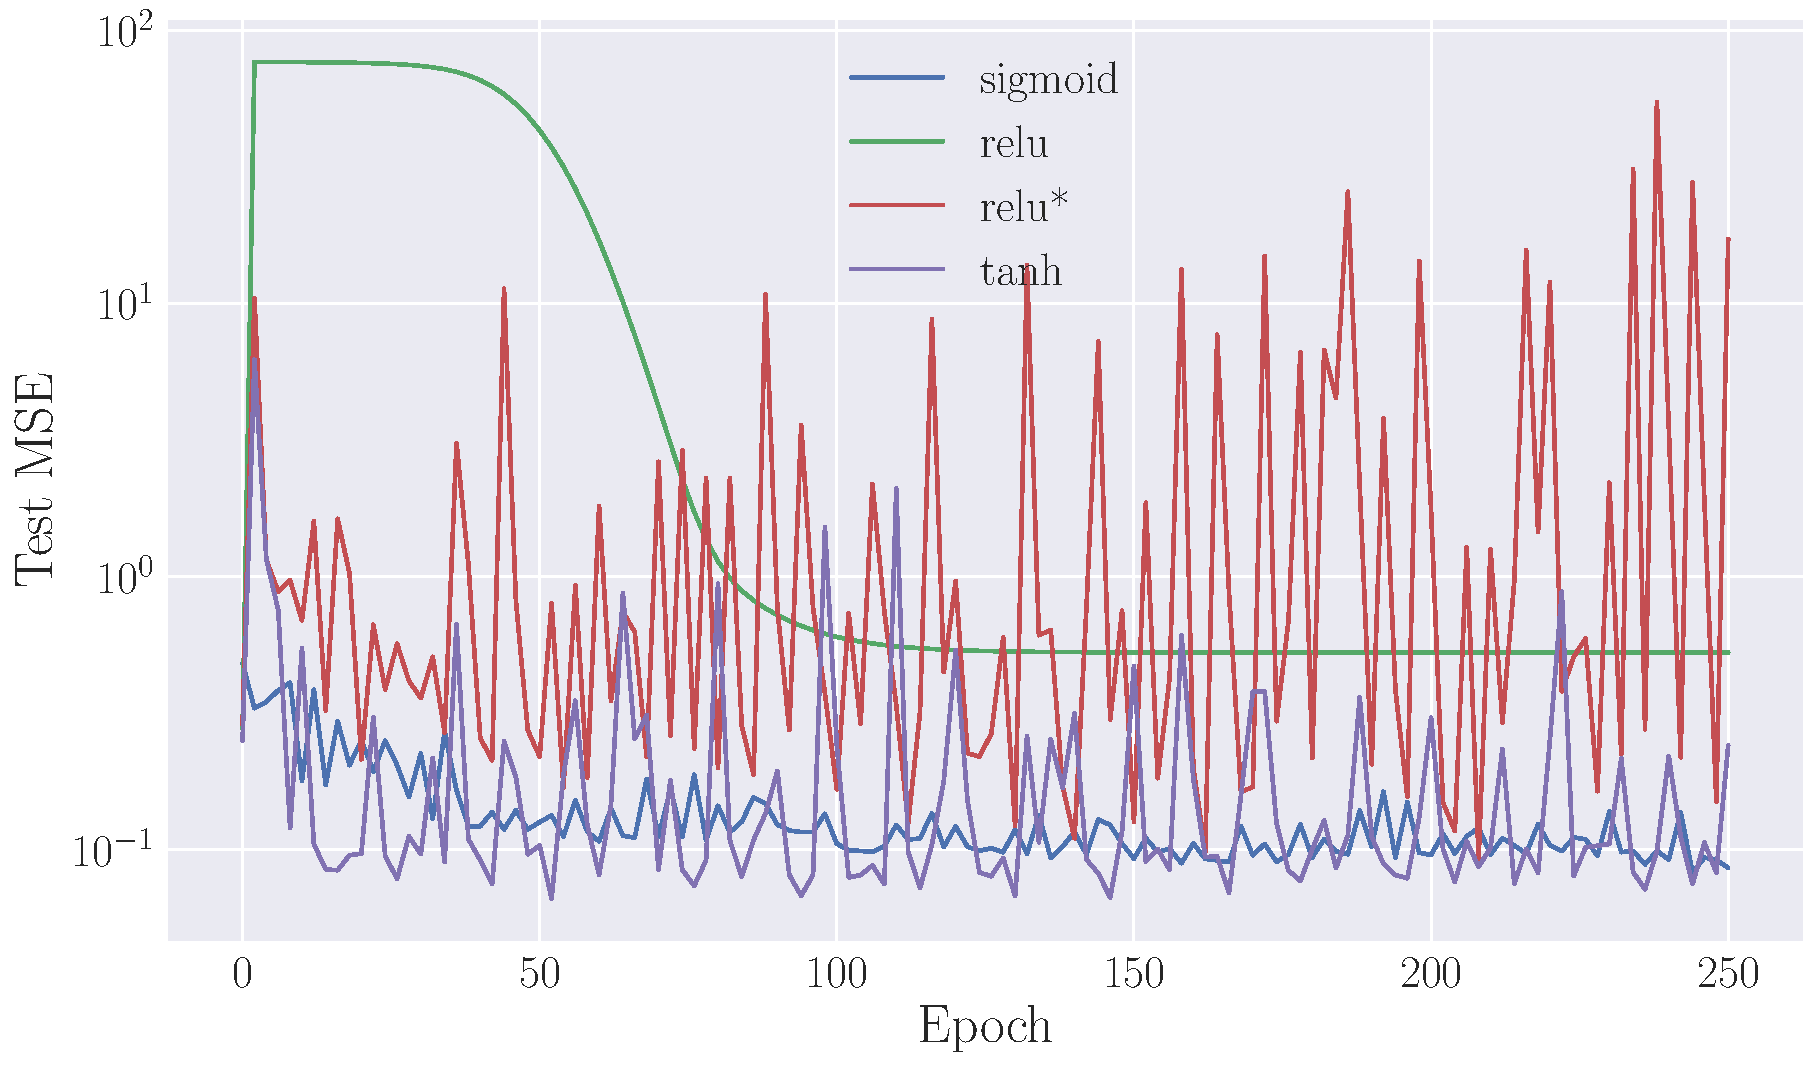
\includegraphics[width=\linewidth]{actFuncPerEpoch.pdf}
    \caption{Plot of the MSE for up to 250 epochs, using SGD with RMSProp as optimiser performing regression analysis with $L-1=1$ hidden layer with $N_l=30$ neurons with $\eta=10^{-1}$ and $\lambda=10^{-4}$. The four different activation functions perform differently. Note the logarithmic MSE axis.}
    \label{fig:reg_act_epoch}
\end{figure}

\begin{figure}[h!]
    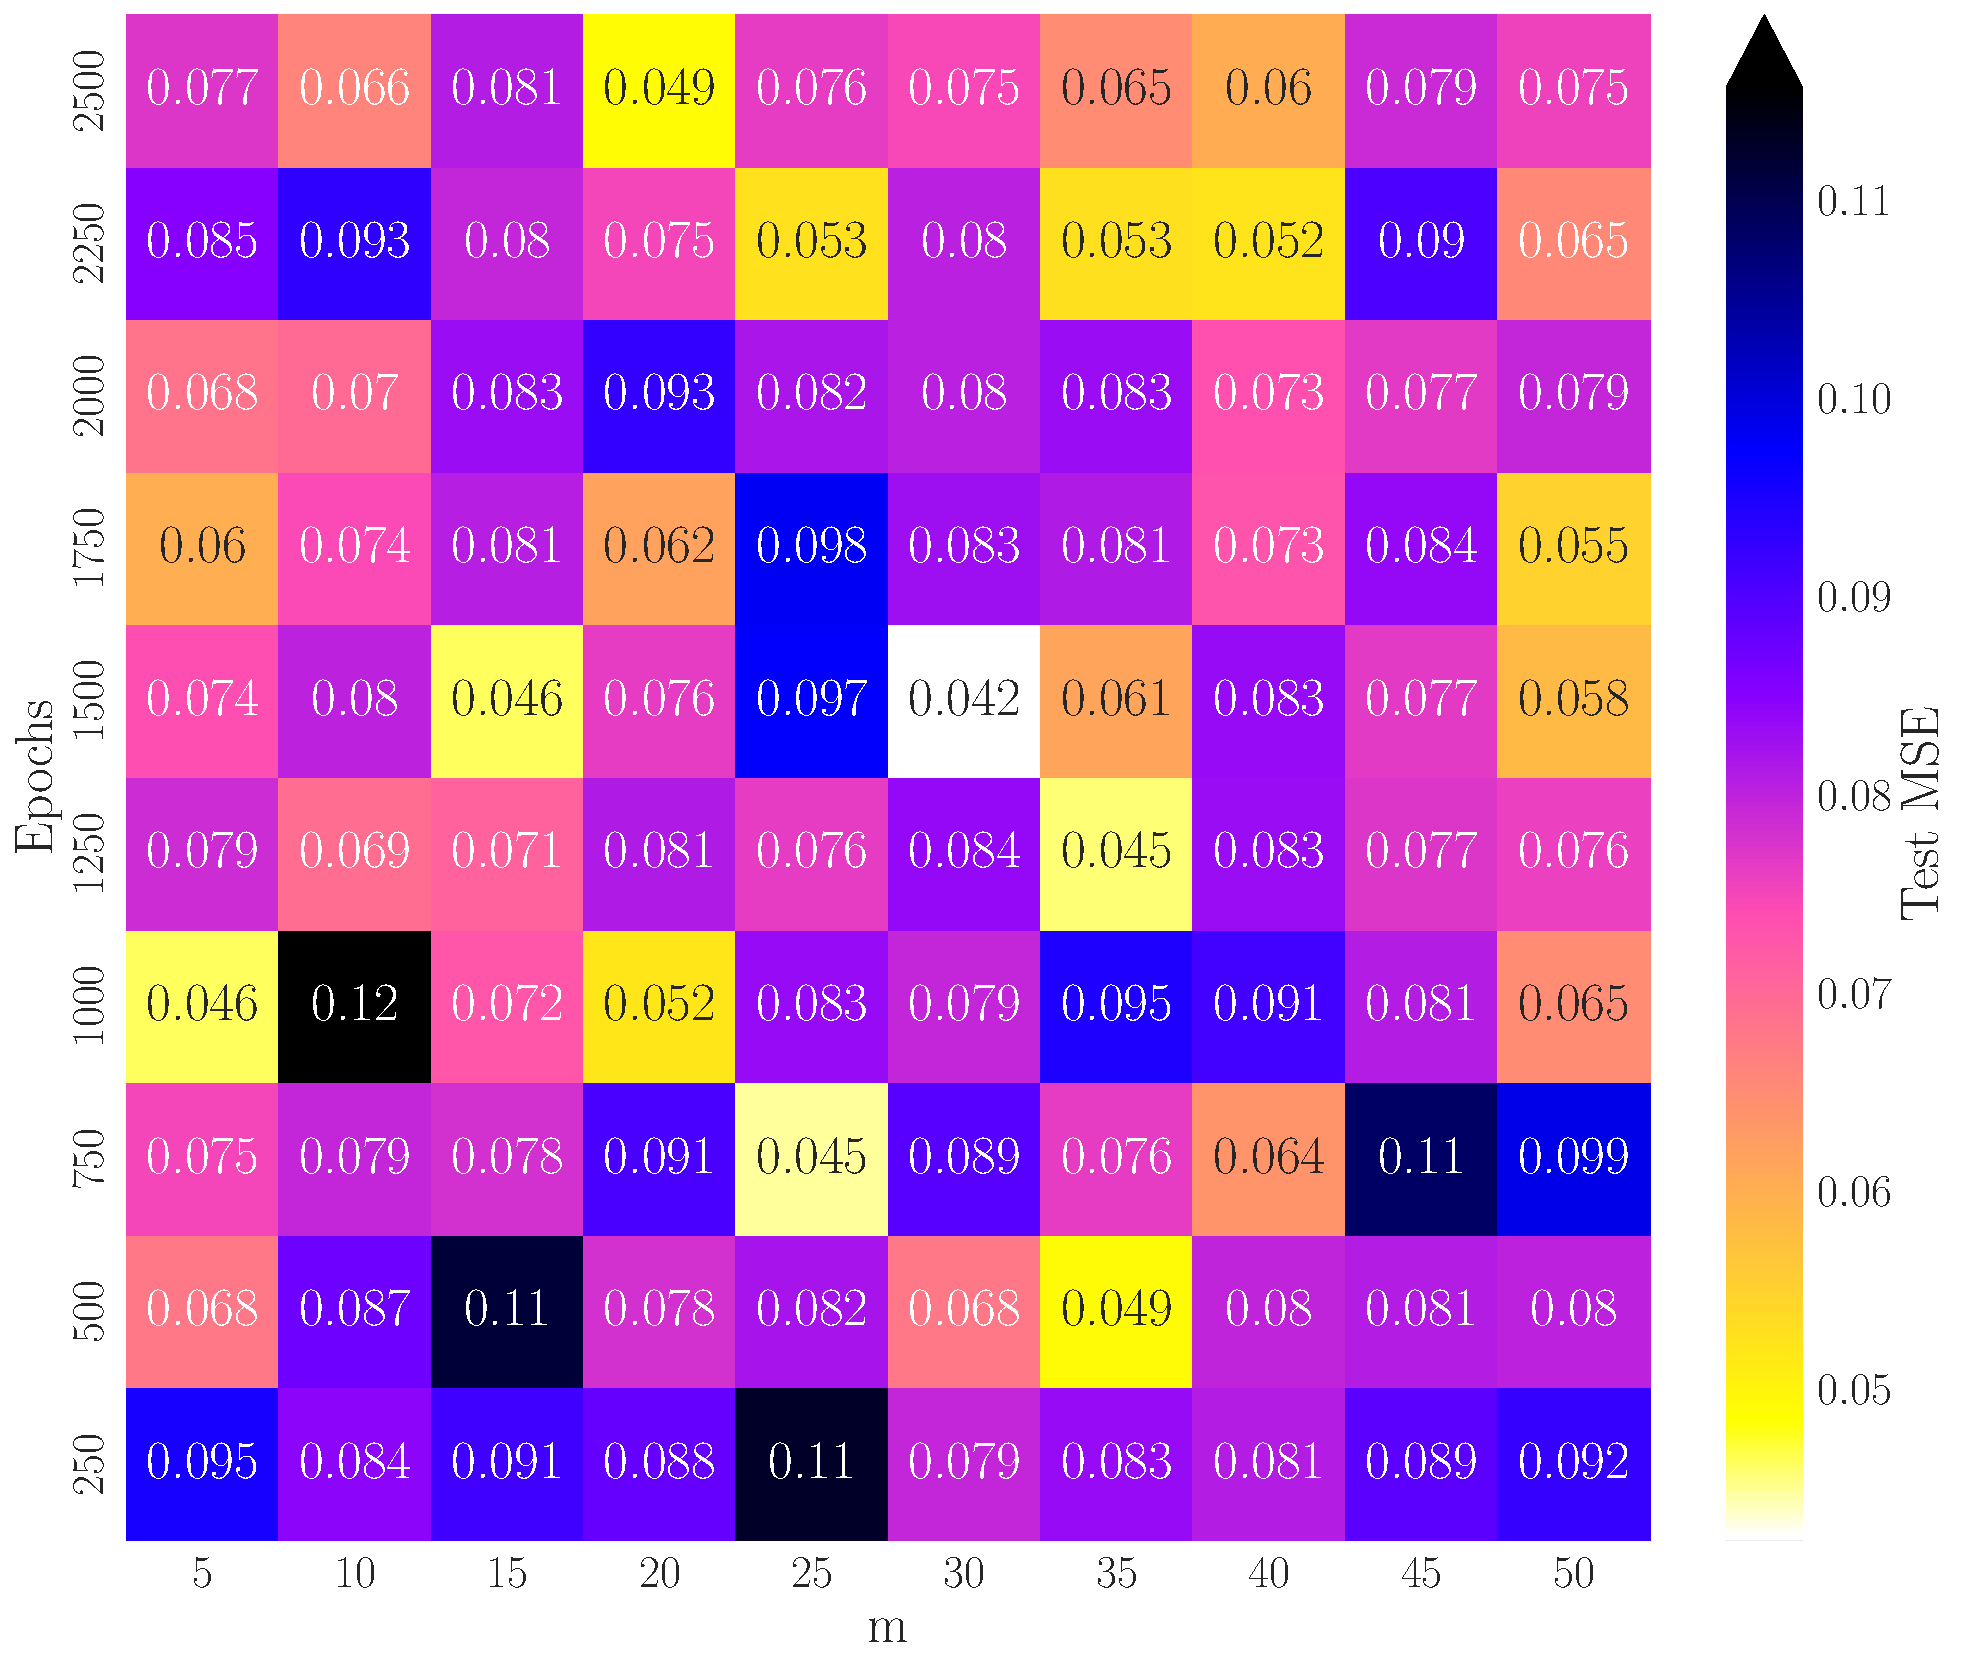
\includegraphics[width=\linewidth]{epoch_minibatch_analysis.pdf}
    \caption{Heatmap of the MSE as function of the number of minibatches $m$ and training epochs, using SGD with RMSProp as optimiser performing regression analysis with $L-1=1$ hidden layer with $N_l=30$ neurons with $\eta=10^{-1}$ and $\lambda=10^{-4}$ using sigmoid as activation function. }
    \label{fig:reg_minibatch_epoch}
\end{figure}




\clearpage

\section{Classification figures}\label{app:classification}

\begin{figure}[h!]
    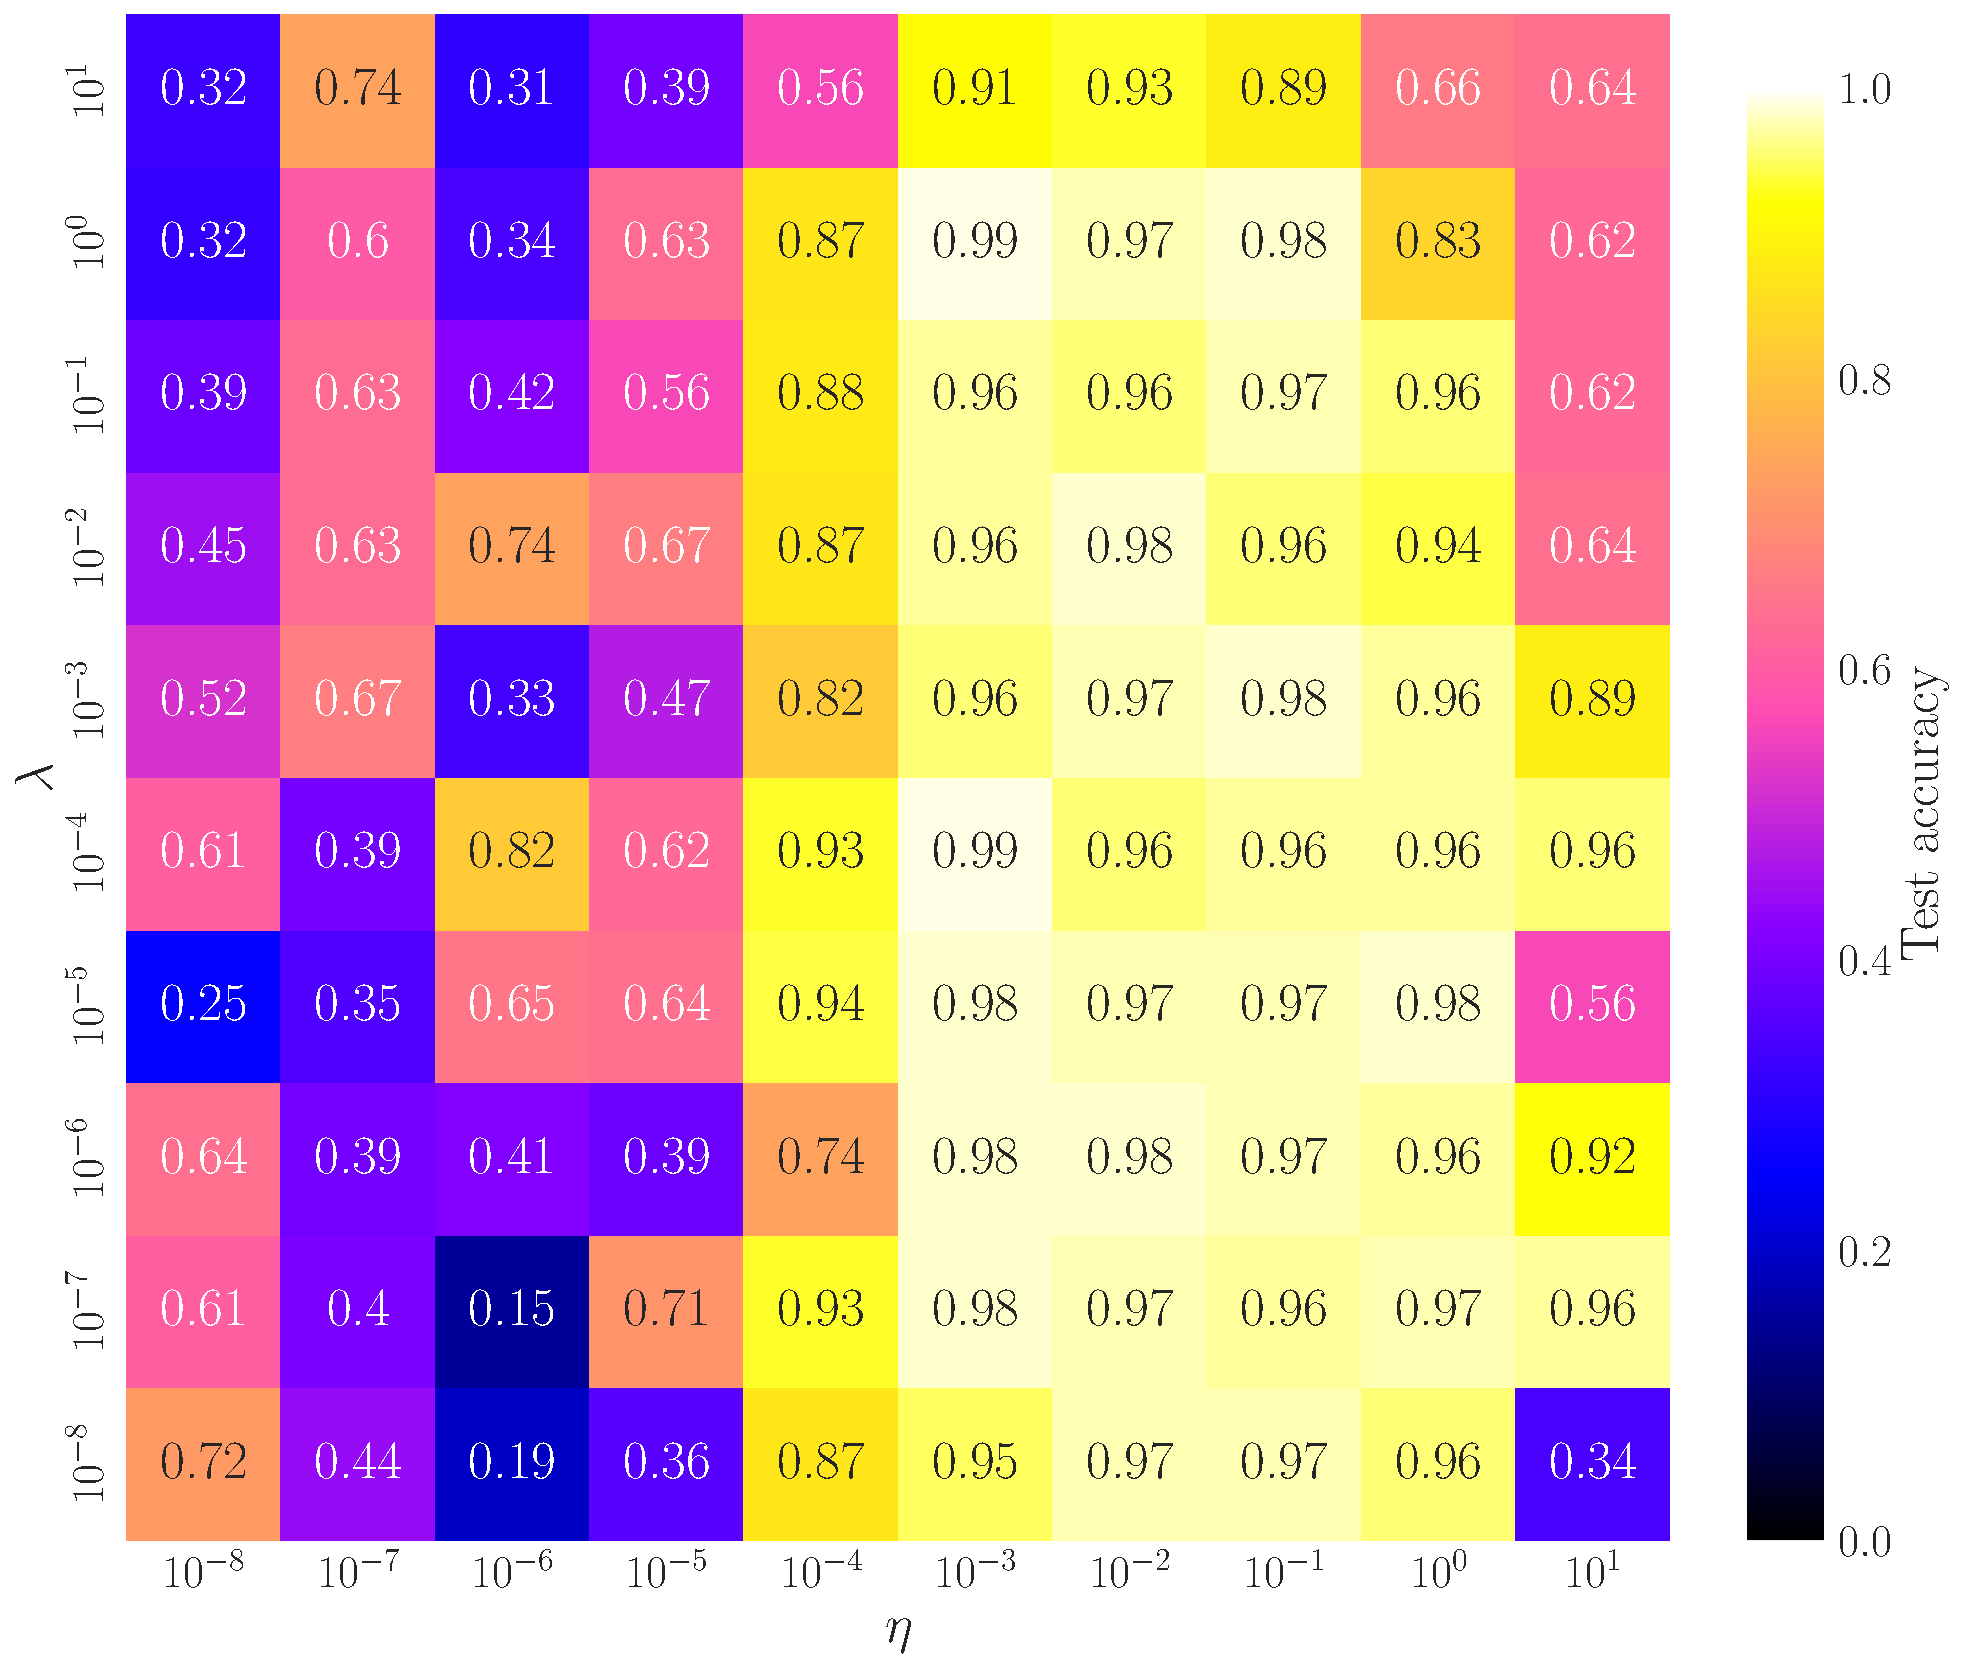
\includegraphics[width=\linewidth]{eta_lambda_analysisCancer.pdf}
    \caption{Heatmap of accuracy as function of learning rate $\eta$ and regularisation parameter $\lambda$, using SGD with RMSProp as optimiser performing regression analysis of a 3 layered, 15-10-5 neurons, neural network. }
    \label{fig:class_eta_lambda}
\end{figure}

\begin{figure}[h!]
    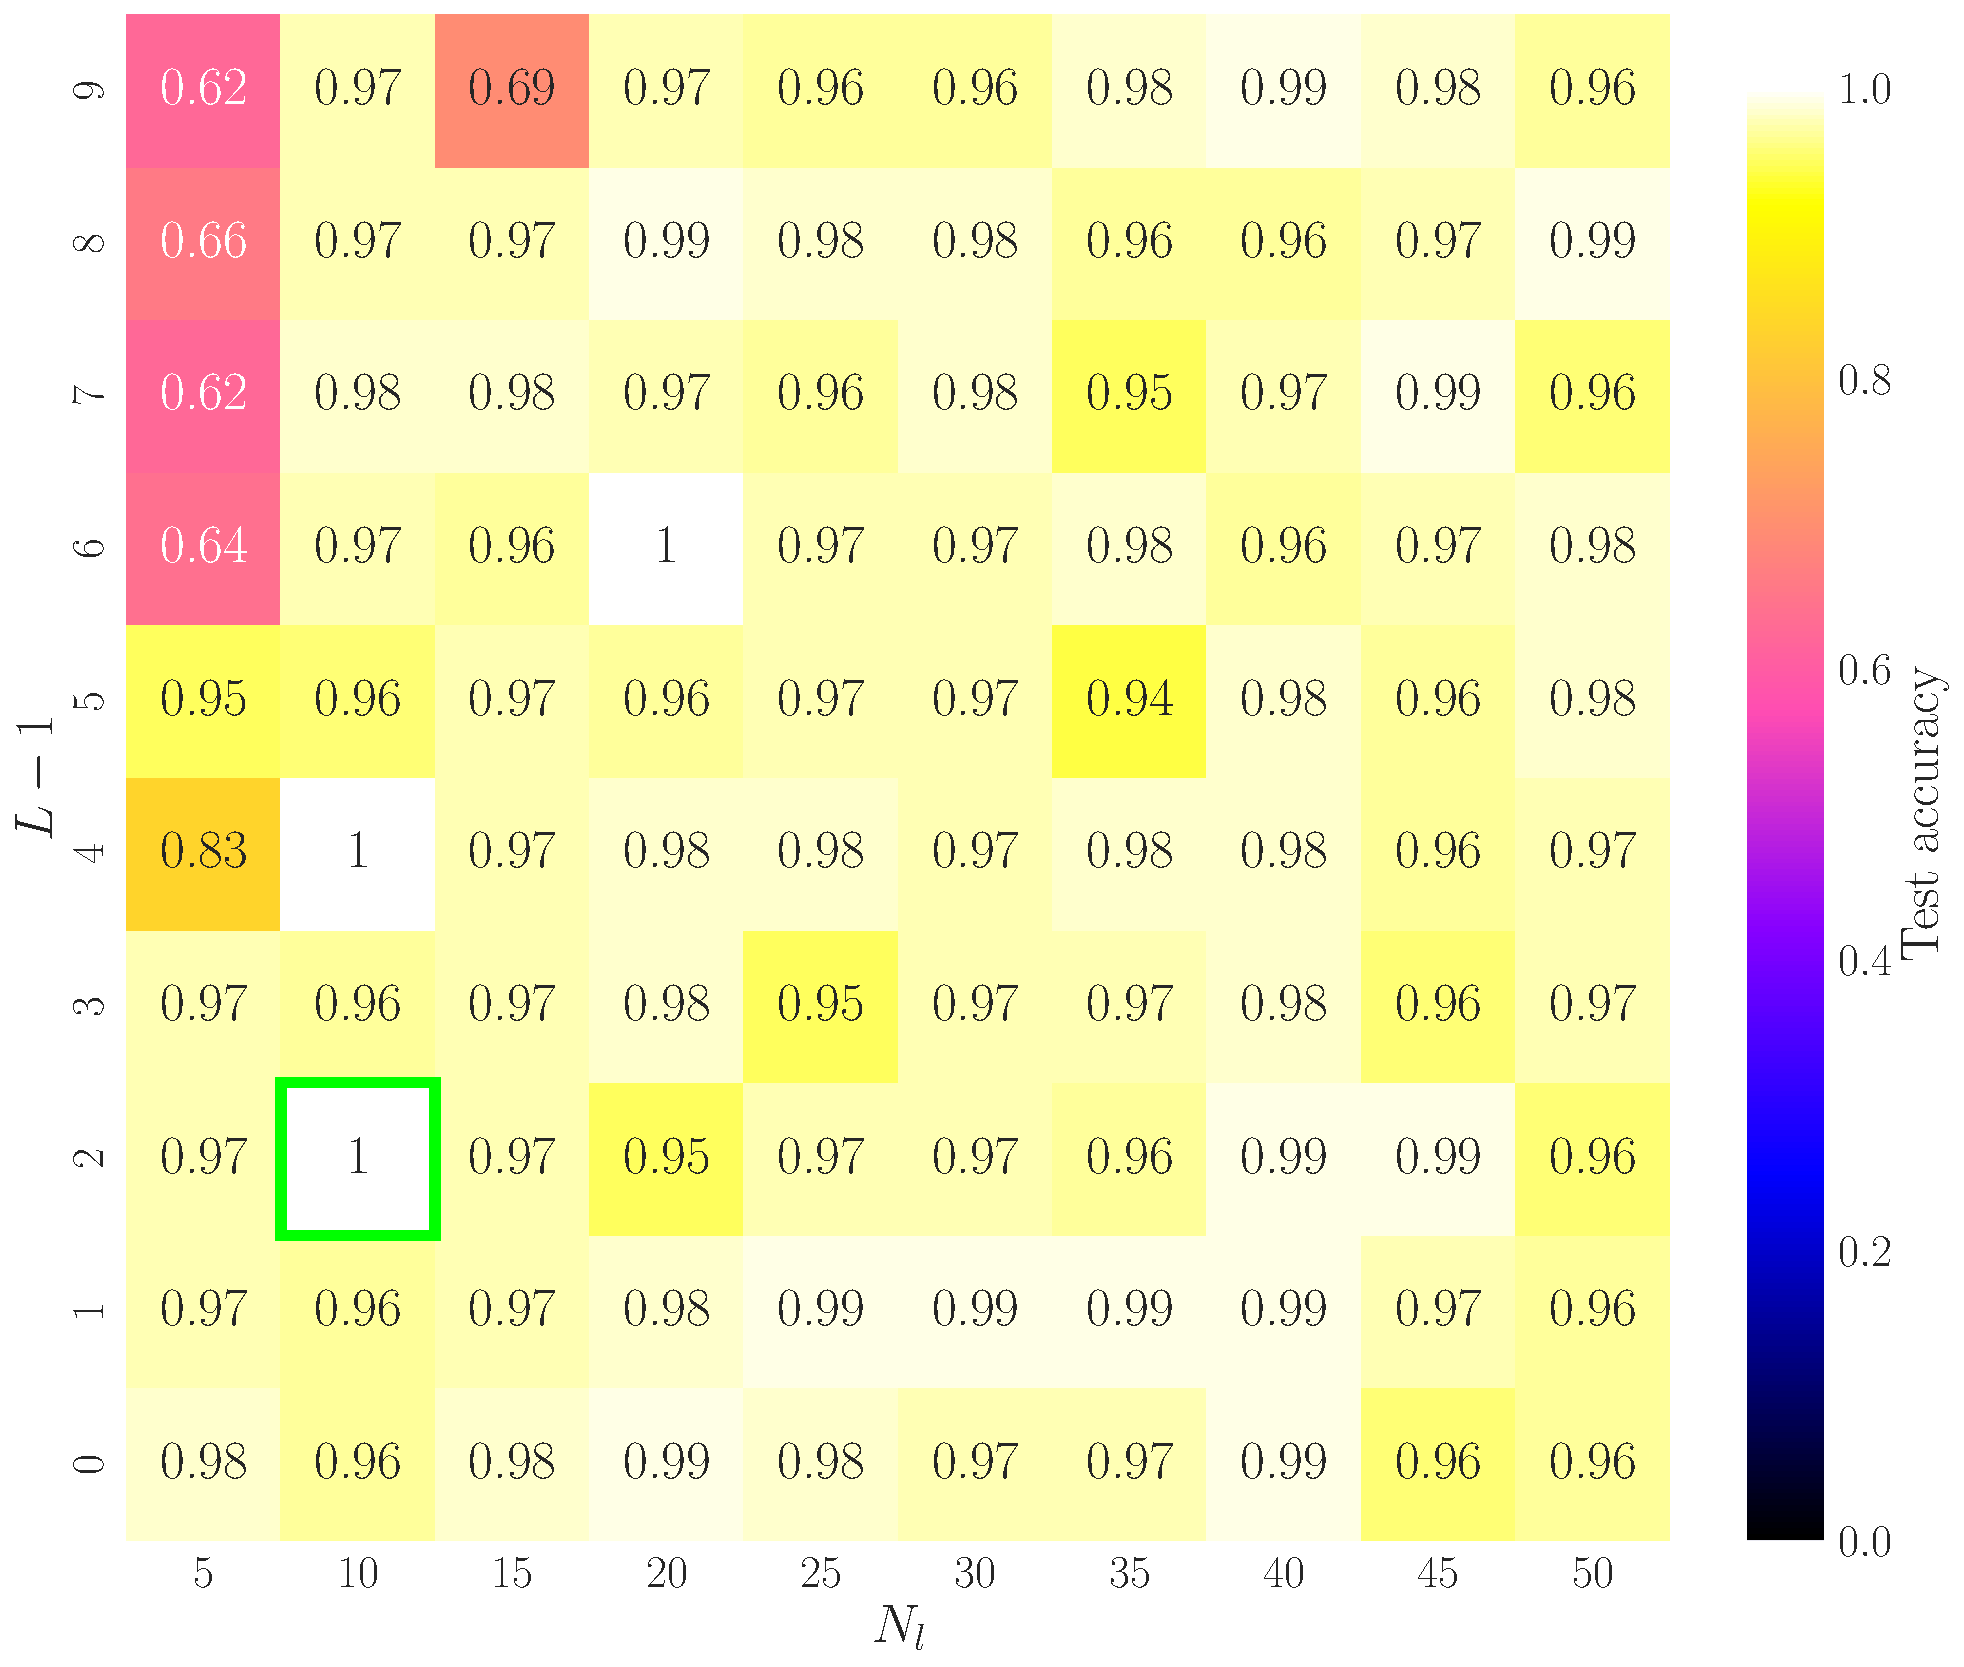
\includegraphics[width=\linewidth]{layer_neuron_analysisCancer.pdf}
    \caption{Heatmap of accuracy as function of hidden layers $L-1$ and neurons per layer $N_l$, using SGD with RMSProp as optimiser performing regression analysis with $\eta=10^{-3}$ and $\lambda=10^{-6}$.}
    \label{fig:class_layer_neuron}
\end{figure}

\begin{figure}[h!]
    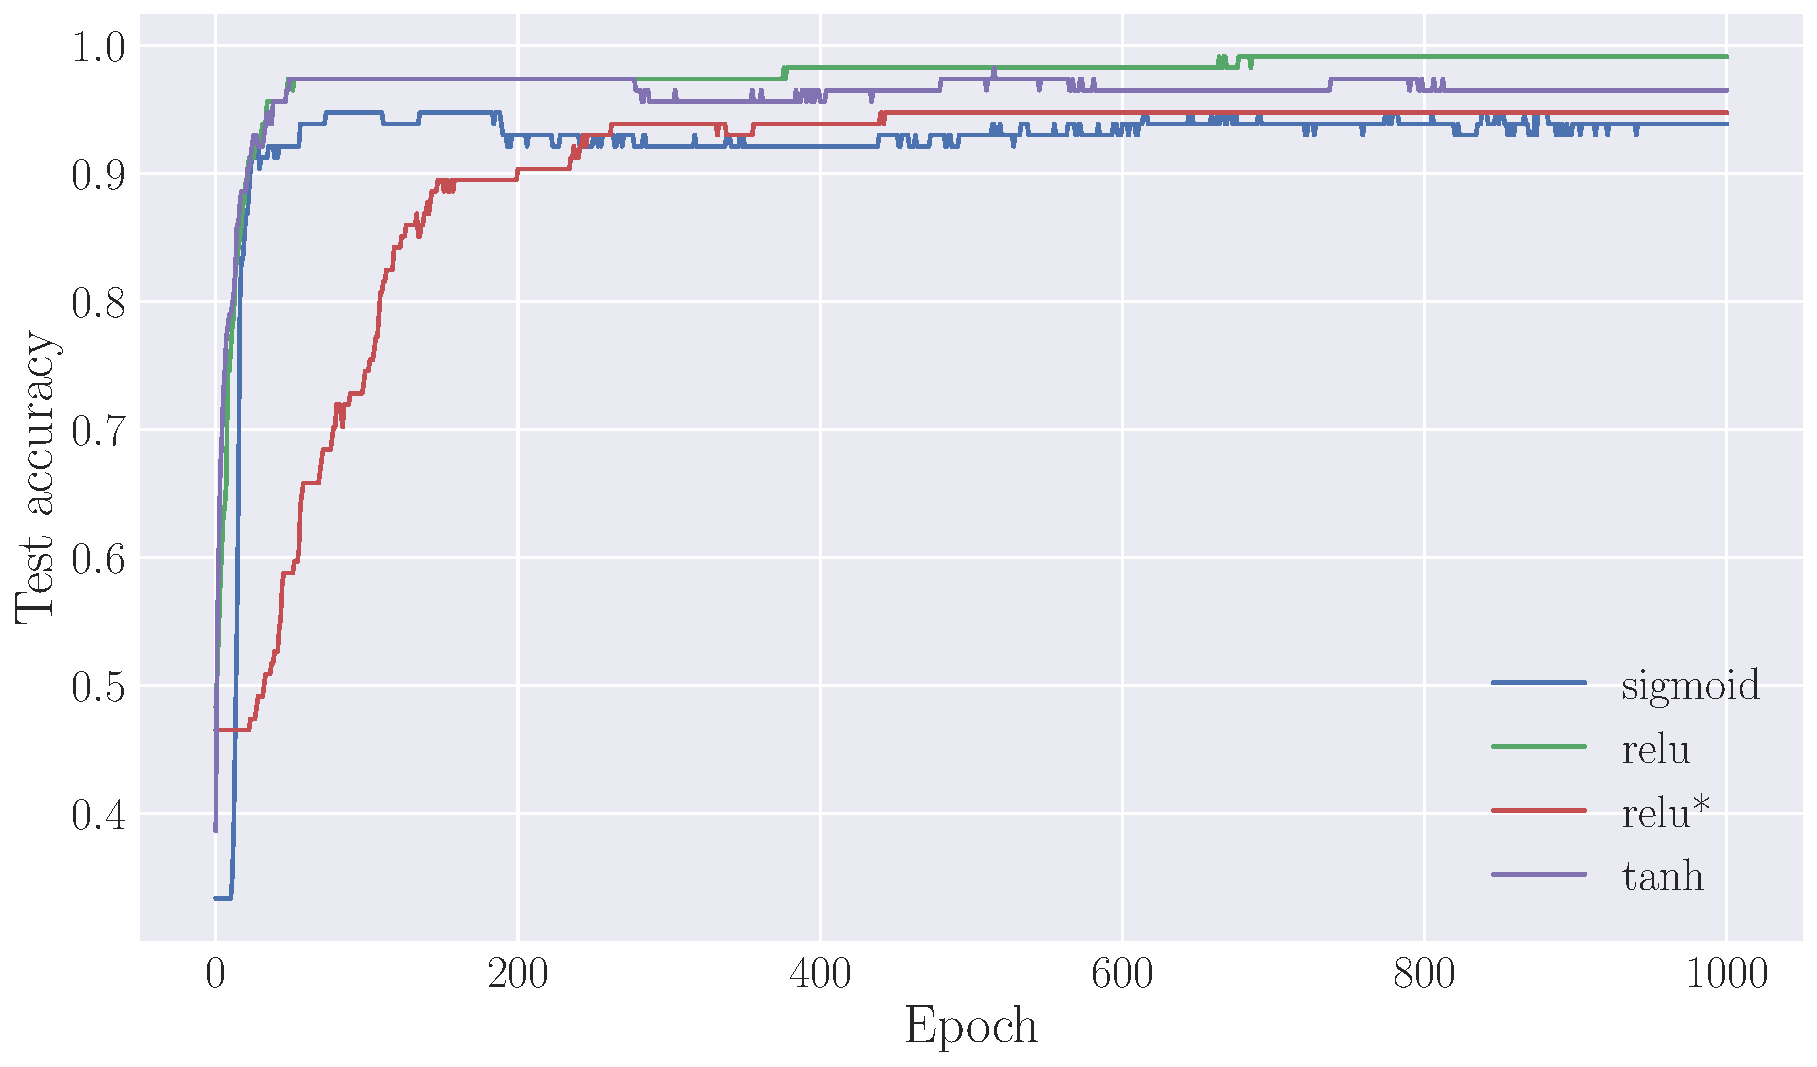
\includegraphics[width=\linewidth]{actFuncPerEpoch1000Cancer.pdf}
    \caption{Plot of accuracy for up to 1000 epochs, using SGD with RMSProp as optimiser performing regression analysis with $L-1=2$ hidden layers with $N_l=10$ neurons each with $\eta=10^{-3}$ and $\lambda=10^{-6}$. The four different activation functions perform differently.}
    \label{fig:class_act_epoch1000}
\end{figure}

\begin{figure}[h!]
    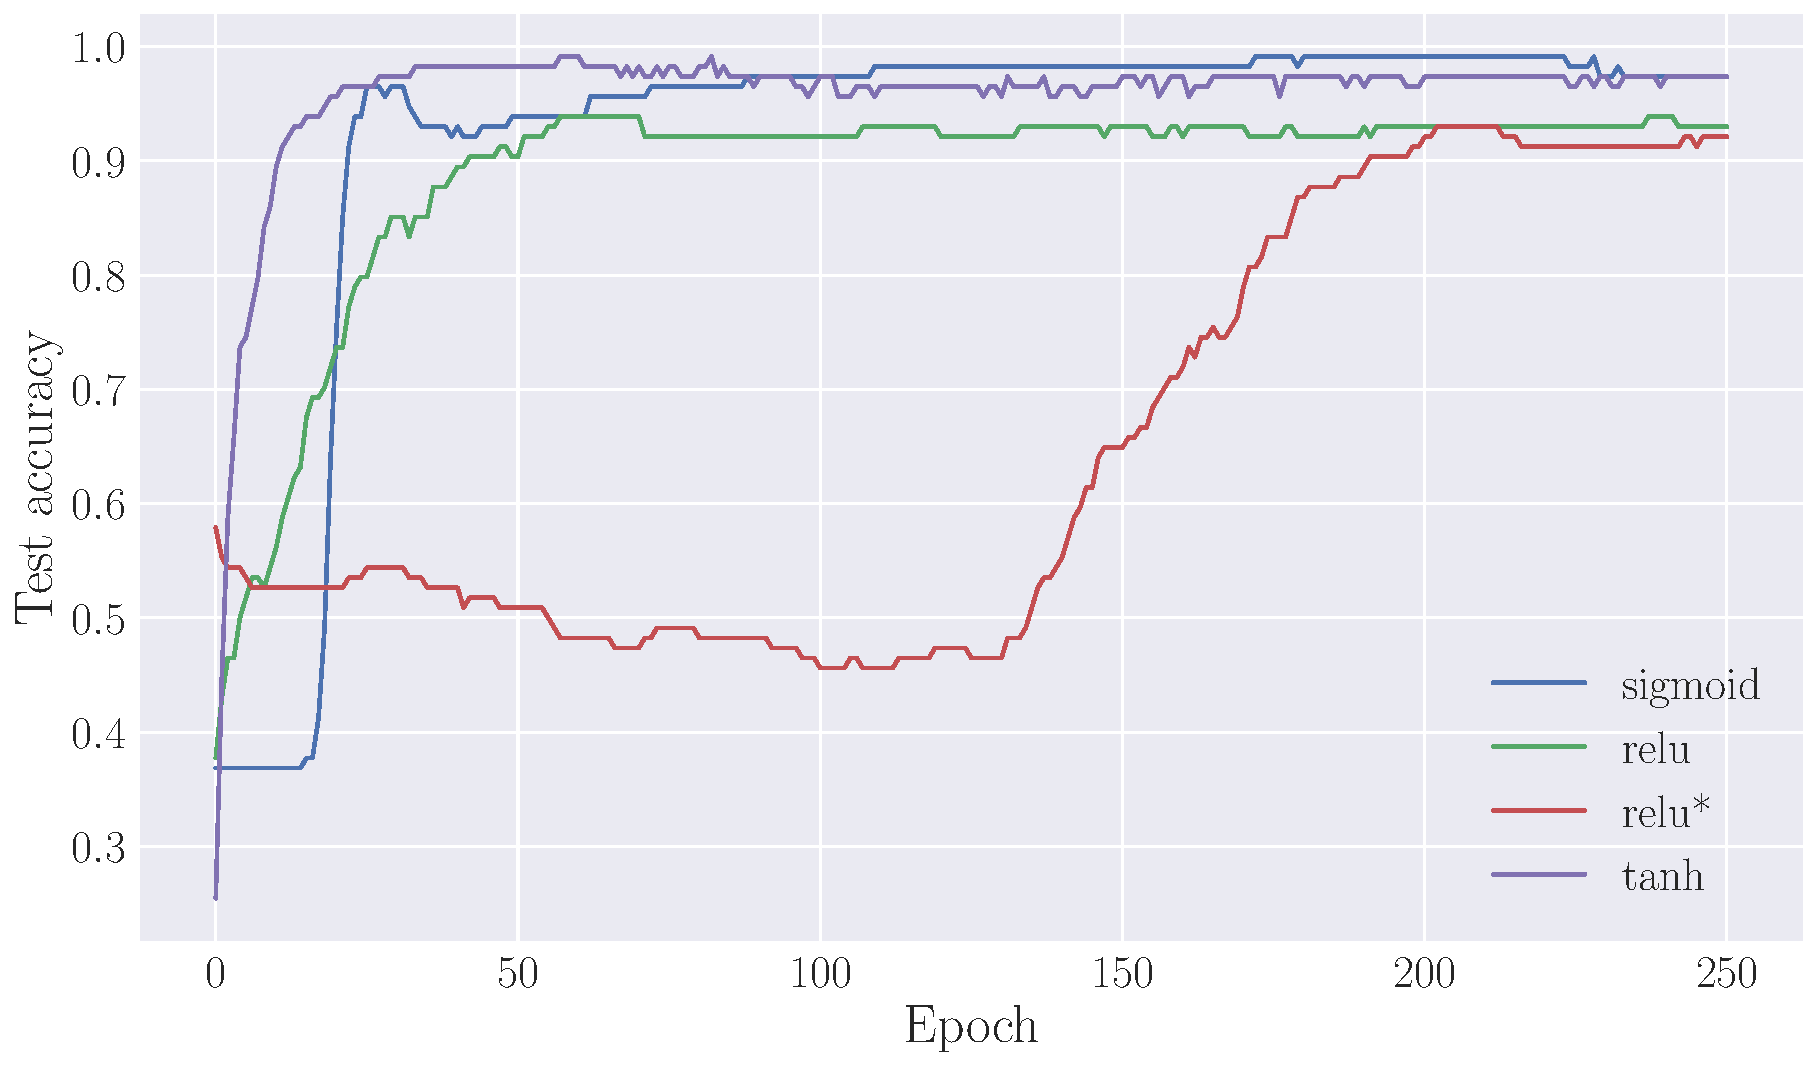
\includegraphics[width=\linewidth]{actFuncPerEpochCancer.pdf}
    \caption{Plot of accuracy for up to 250 epochs, using SGD with RMSProp as optimiser performing regression analysis with $L-1=2$ hidden layer with $N_l=10$ neurons with $\eta=10^{-3}$ and $\lambda=10^{-6}$. The four different activation functions perform differently.}
    \label{fig:class_act_epoch}
\end{figure}

\begin{figure}[h!]
    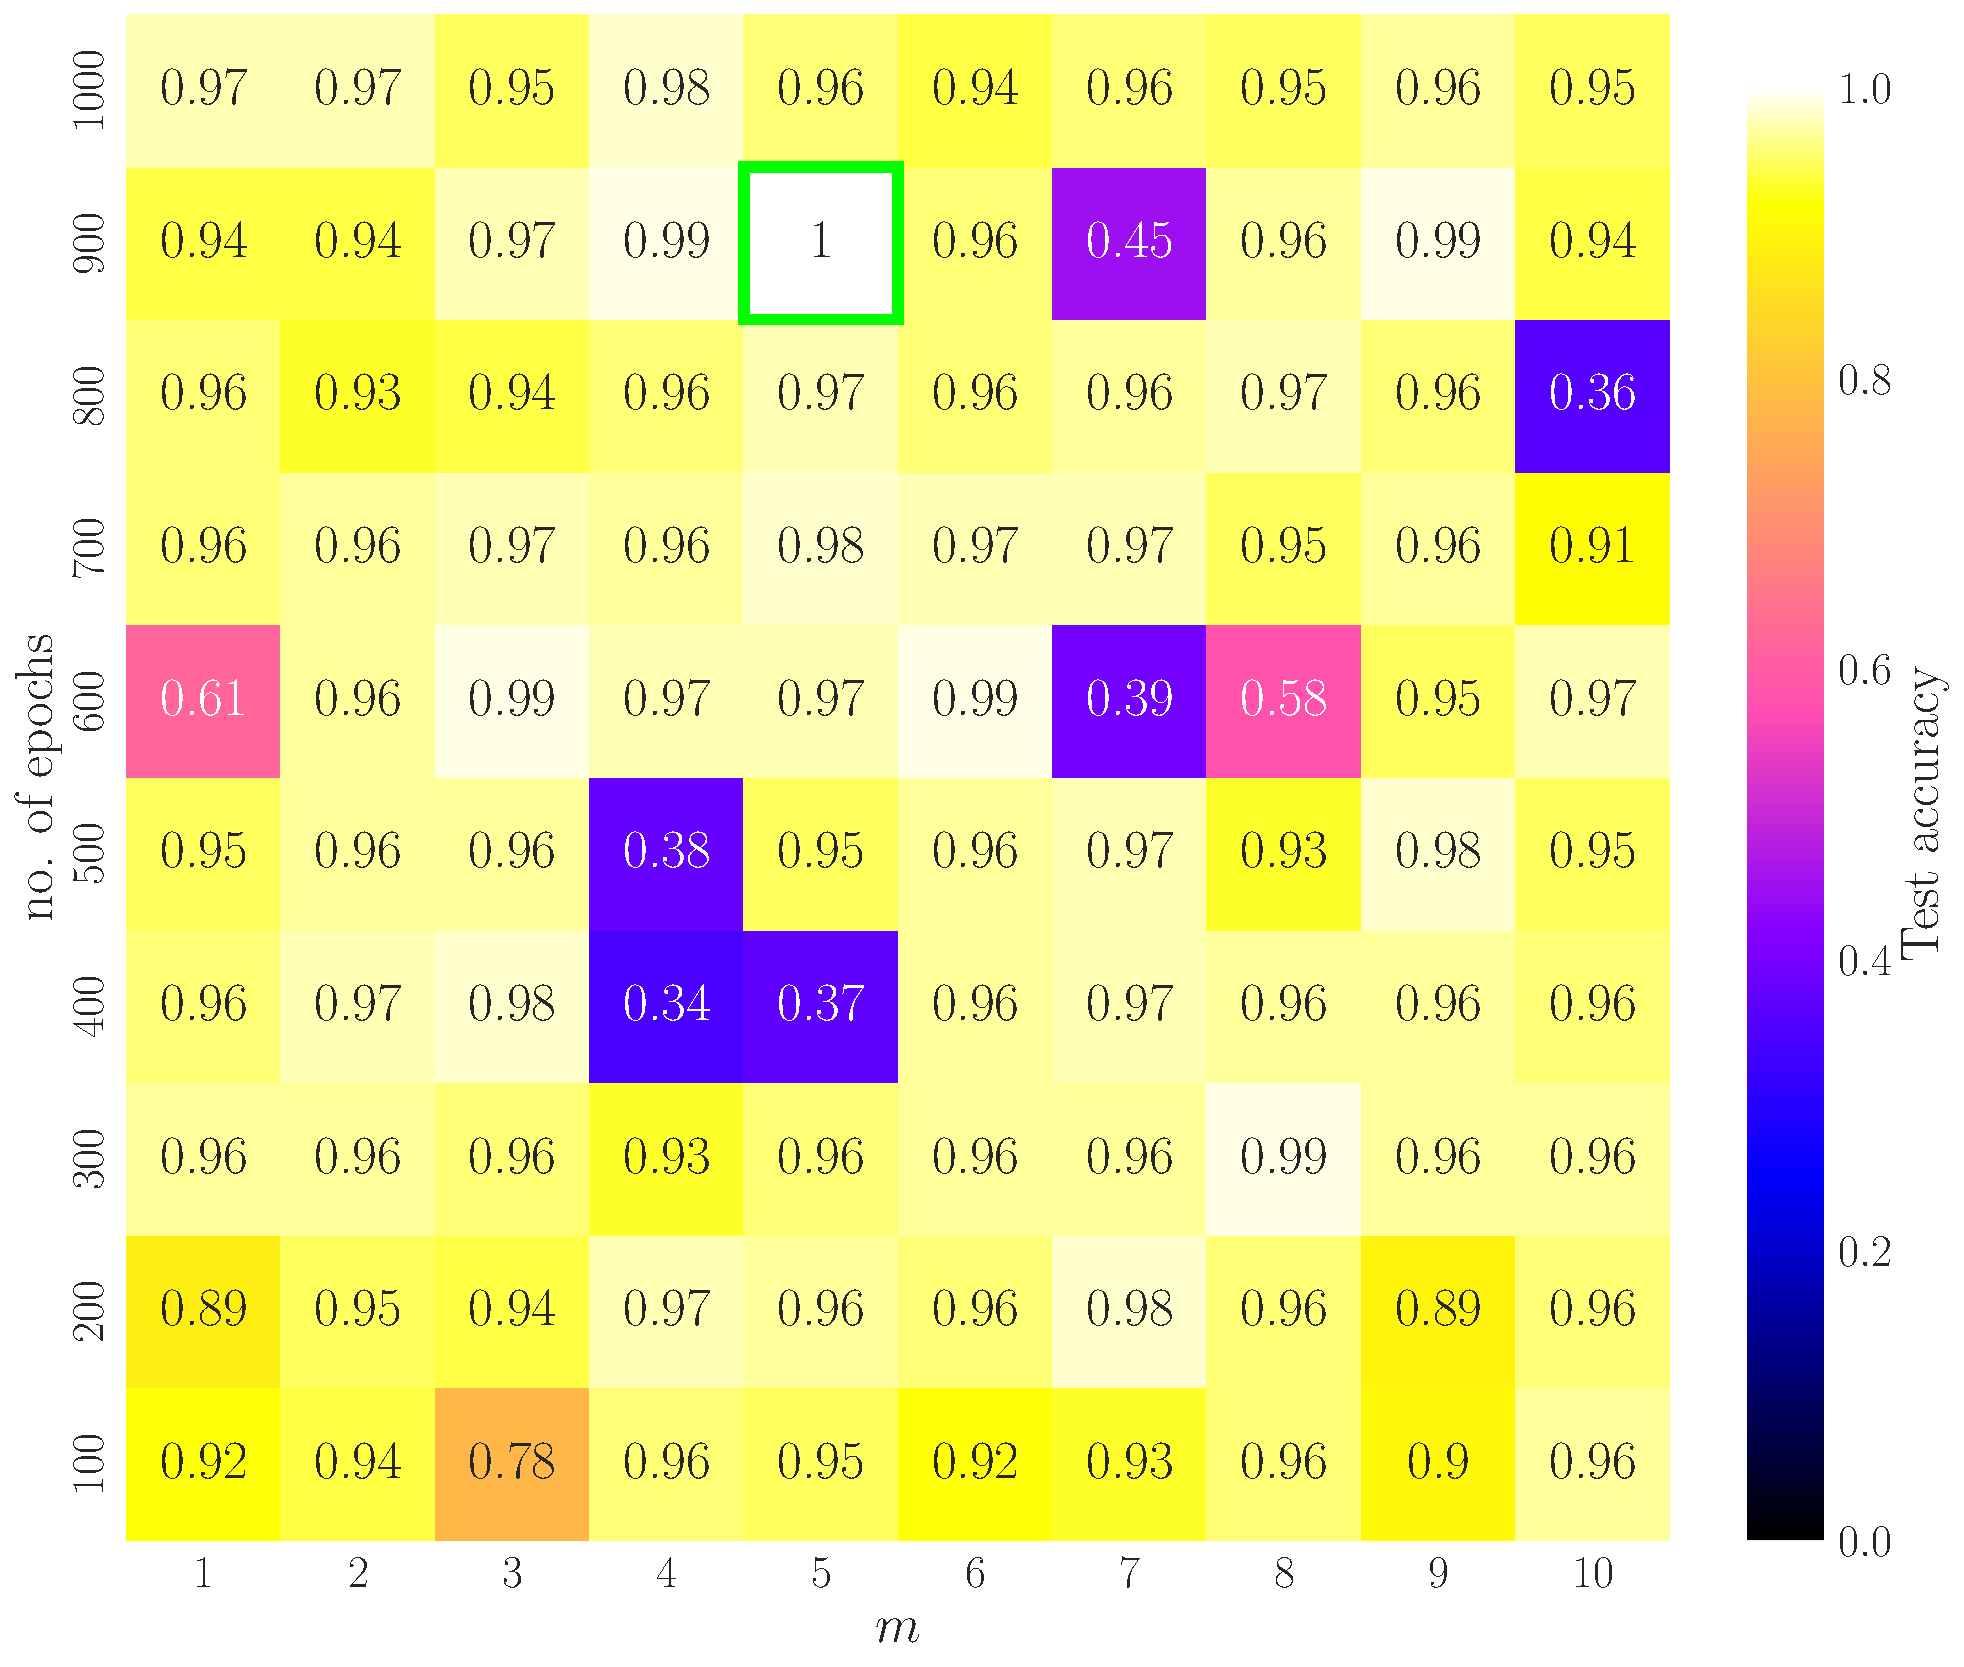
\includegraphics[width=\linewidth]{epoch_minibatch_analysisCancer.pdf}
    \caption{Heatmap of accuracy as function of the number of minibatches $m$ and training epochs, using SGD with RMSProp as optimiser performing regression analysis with $L-1=2$ hidden layer with $N_l=10$ neurons with $\eta=10^{-3}$ and $\lambda=10^{-6}$ using RELU as activation function. }
    \label{fig:class_minibatch_epoch}
\end{figure}


\clearpage

\section{Logistic regression figure}\label{app:logistic}

\begin{figure}[h!]
    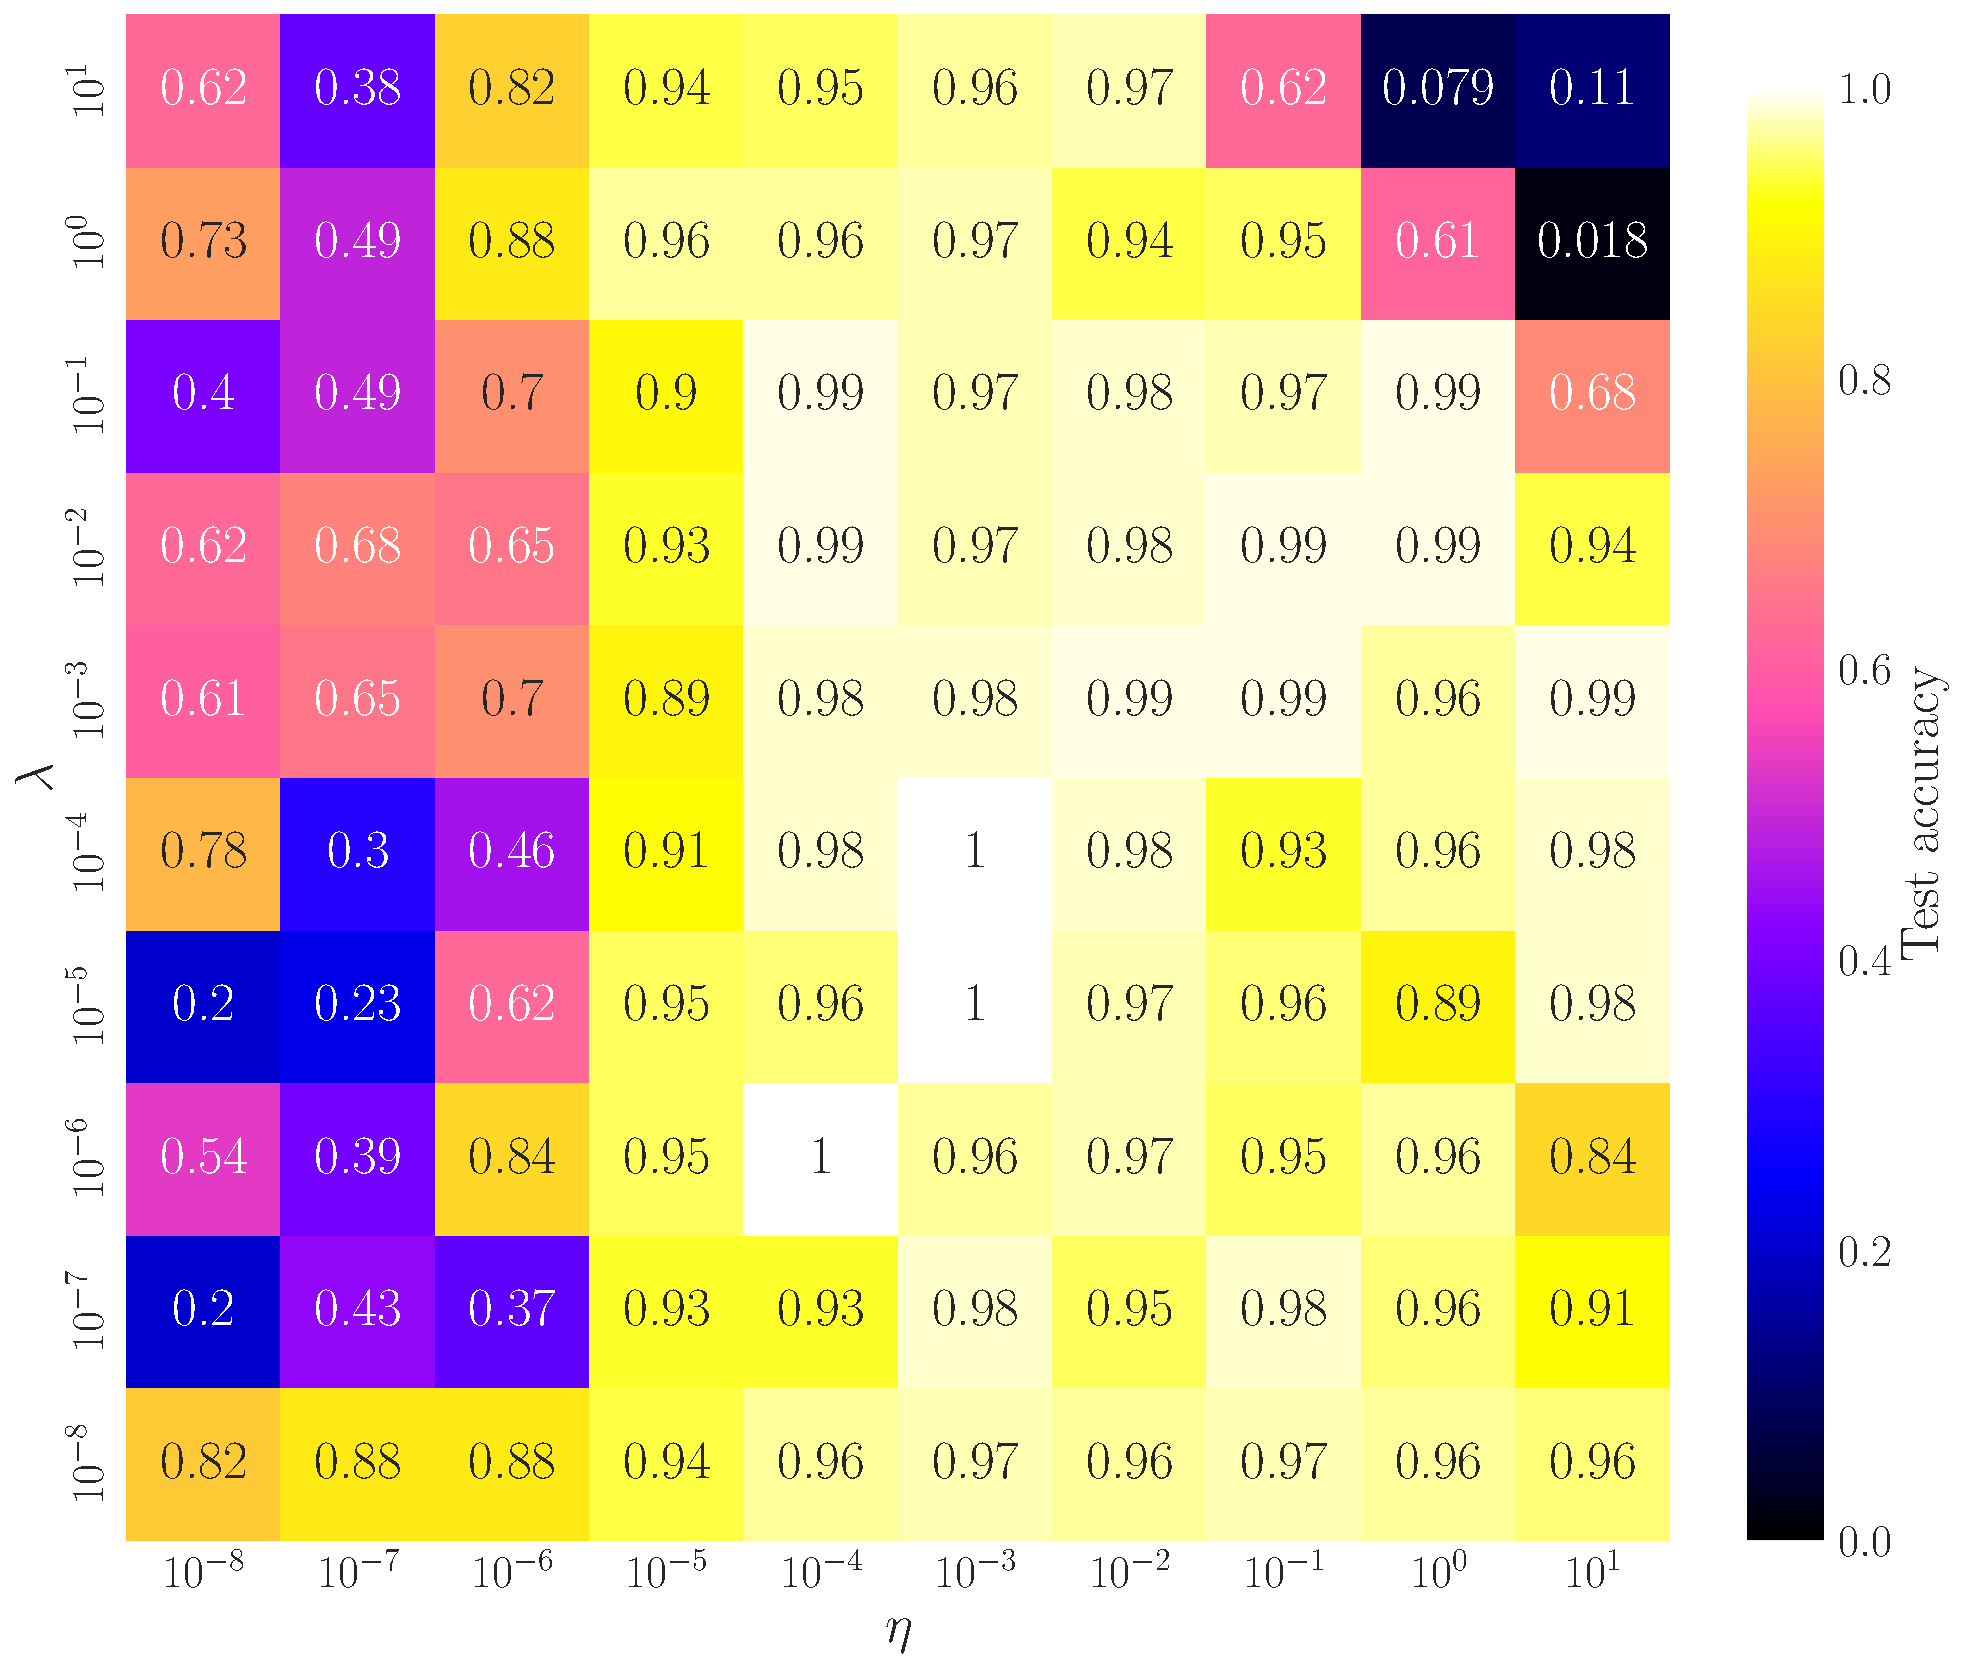
\includegraphics[width=\linewidth]{logistic.pdf}
    \caption{Heatmap of the MSE as function of learning rate $\eta$ and regularisation parameter $\lambda$, using SGD with RMSProp as optimiser performing regression analysis of a network with no hidden layers using the sigmoid function as activation function. This is equivalent of performing logistic regression.}
    \label{fig:logistic_eta_lambda}
\end{figure}


\clearpage

\section{Optimiser algorithms}\label{app:optimisers}

\checkthis{FIX CITATIONS}

Adagrad\footnote{Algorithm 8.4 in Goodfellow et al.}

\begin{algorithm}
\caption{Adagrad algorithm}\label{algo:adagrad}
\begin{algorithmic}
    \Require Global learning rate $\eta$
    \Require Initial parameter $\svec{\theta}$
    \Ensure Initialise gradient accumulation variable $\vec{r} = \vec{0}$
    \While{$\abs{\vec{v}}>10^{-10}$}
        \State Accumulate squared gradient: $\vec{r} \leftarrow \vec{r} + \vec{g}\odot\vec{g}$
        \State Compute update 
    \EndWhile
\end{algorithmic}
\end{algorithm}




\section{Back propagation algorithm}\label{app:backprop}
    The output $\vec{\hat{y}}$ of our NN is given by the layer value of the output layer $\vec{h}^L$ passed through an output function $g_L$: $\vec{\hat{y}} = g_L(\vec{h}^L)$. The output error is given by
    \begin{equation}\label{eq:app_backprop_output_error}
        \svec{\delta}^L = \dv{g_L(\vec{a}^L)}{\vec{a}^L} \odot \pdv{\mathcal{L}}{\vec{\hat{y}}} =\dv{g_L(\vec{a}^L)}{\vec{a}^L} \odot \pdv{\mathcal{L}}{\vec{h}^L}\left( \pdv{\vec{\hat{y}}}{\vec{h}^L} \right)^{-1},
    \end{equation}
    where $\odot$ is the element wise Hadamard product. This error is propagated through the layers of the network in backward order,
    \begin{equation}\label{eq:app_backprop_prop_error}
        \svec{\delta}^l = \svec{\delta}^{l+1}W^{l+1\!\to l} \odot \dv{}{\vec{a}^l}g_l(\vec{a}^l),
    \end{equation}
    for $l=L-1, L-2,\dots, 1$. Having found the error propagated through each layer, we update the weights and biases as follows:
    \begin{equation}\label{eq:app_backprop_update}
        \begin{split}
            \nabla_{\!W}^l &= (\svec{\delta}^l)\TT\vec{h}^{l-1} \\
            \nabla_{\!b}^l &= \svec{\delta}^l \\
            W^l &= \mathcal{U}(W^l, \nabla_{\!W}^l)\\
            \vec{b}^l &= \mathcal{U}(\vec{b}^l, \nabla_{\!b}^l) \\
            \implies \svec{\theta}^l &= \mathcal{U}(\svec{\theta}^l, \nabla_{\!\theta}^l) \,;\quad\quad\quad \svec{\theta}^l = (W^l, \vec{b}^l)
,        \end{split}
    \end{equation}
    Here $\mathcal{U}(\svec{\theta}, \nabla_{\!\theta})$ is a function that updates the parameter $\svec{\theta}$ according som some optimisation scheme, typically SGD with a favoured optimised. For reference, plain gradient descent reads: $\mathcal{U}(\svec{\theta}, \nabla_{\!\theta}) = \svec{\theta} - \eta\nabla_{\!\theta}$, where $\eta$ is the learning rate. 


